\documentclass{exercise}

\institute{Lehr- und Forschungsgebiet Kontinuumsmechanik}
\title{Übung 7}
\author{Joshua Feld, 406718}
\course{Mechanik verformbarer Körper}
\professor{Itskov}
\semester{Sommersemester 2022}
\program{CES (Bachelor)}

\begin{document}
    \maketitle

    
    \section*{Aufgabe 1}

    \begin{problem}
        \begin{enumerate}
            \item Ein gehärteter (spröder) Bolzen aus Stahl mit einer Zugfestigkeit \(R_{m, a}\) unterliegt einer kombinierten statischen Zug und Torsionsbeanspruchung.
            Durch Messungen wurde die Zugspannung \(\sigma_x\) und die Scherspannung \(\tau_{xy}\) ermittelt.
            Berechnen Sie die Vergleichsspannungen nach der Normalspannungshypothese und ermitteln Sie die Sicherheit gegen Bruch \(S_B\).
            \item Der unter a) gegebene Bolzen wird zum Erreichen eines zäheren (duktileren) Werkstoffverhaltens einer Wärmebehandlung unterzogen, wodurch sich eine veränderte Zugfestigkeit \(R_{m, b}\) und nunmehr auch eine Streckgrenze \(R_e\) ergeben.
            Die mechanische Belastung sei unverändert.
            Berechnen Sie die Vergleichsspannung nach der Schubspannungshypothese und ermitteln Sie die Sicherheit gegen Fließen \(S_{F, b}\).
            \item Für den unter b) betrachteten Bolzen soll bei unveränderter Belastung die Vergleichsspannung nach der Gestaltänderungsenergiehypothese berechnet werden.
            Ermitteln Sie die Sicherheit gegen Fließen \(S_{F, c}\) und interpretieren Sie die Ergebnisse von Fall b) und c).
        \end{enumerate}
        Gegeben: \(\sigma_x = 450\sis{\mega\pascal}\), \(\tau_{xy} = 300\sis{\mega\pascal}\), \(R_{m, a} = 2000\sis{\mega\pascal}\), \(R_{m, b} = 940\sis{\mega\pascal}\), \(R_e = 700\sis{\mega\pascal}\)
    \end{problem}

    \subsection*{Lösung}
    Die Hauptspannungen ergeben sich aus
    \[
        \sigma_{1, 2} = \frac{\sigma_x + \sigma_y}{2} \pm \sqrt{\parentheses*{\frac{\sigma_x - \sigma_y}{2}}^2 + \tau_{xy}^2}
    \]
    mit \(\sigma_y = 0\) zu
    \[
        \sigma_1 = 600\sis{\mega\pascal}, \quad \sigma_2 = -150\sis{\mega\pascal}.
    \]
    \begin{enumerate}
        \item Der Vergleichsspannungswert gemäß der Normalspannungshypothese ergibt sich zu
        \[
            \sigma_{V, N} = \sigma_1 = 600\sis{\mega\pascal}.
        \]
        Für die Sicherheit gegen Bruch ergibt sich
        \[
            S_B = \frac{R_{m, a}}{\sigma_{V, N}} = \frac{10}{3} > 1.
        \]
        \item Der Vergleichsspannungswert gemäß der Schubspannungshypothese ergibt sich zu
        \[
            \sigma_{V, S} = 2\tau_{\text{max}} = \sqrt{\parentheses*{\sigma_x - \sigma_y}^2 + 4\tau_{xy}^2} = \sigma_1 - \sigma_2 = 750\sis{\mega\pascal}.
        \]
        Für die Sicherheit gegen Fließen ergibt sich
        \[
            S_{F, b} = \frac{R_e}{\sigma_{V, S}} = \frac{14}{15} < 1.
        \]
        \item Der Vergleichsspannungswert gemäß der Hypothese der Gestaltänderungsenergie ergibt sich zu
        \[
            \sigma_{V, G} = \sqrt{\sigma_x^2 + \sigma_y^2 - \sigma_x \sigma_y + 3\tau_{xy}^2} = \sqrt{\sigma_1^2 + \sigma_2^2 - \sigma_1 \sigma_2} = 687,386\sis{\mega\pascal}.
        \]
        Für die Sicherheit gegen Fließen ergibt sich
        \[
            S_{F, c} = \frac{R_e}{\sigma_{V, G}} = 1,018 > 1.
        \]
        Für die Schubspannungshypothese ist die Sicherheit kleiner als \(1\) und somit nicht ausreichend.
        Gemäß der Hypothese der Gestaltungsenergie ist die Sicherheit größer als \(1\) und somit ausreichend.
    \end{enumerate}


    \section*{Aufgabe 2}

    \begin{problem}
        Für einen rechtwinkligen Dreiecksquerschnitt sind die Flächenträgheitsmomente bezüglich der Schwerpunktachsen \(y\) und \(z\) sowie das Deviationsmoment unter Zuhilfename der Integralformeln zu berechnen.
        \begin{center}
            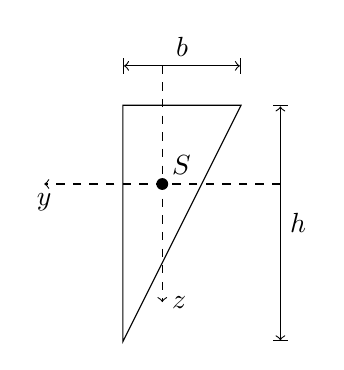
\begin{tikzpicture}
                \draw (0,0) -- (1.5,0) -- (0,-3) -- cycle;
                \fill (.5,-1) circle (.75mm) node[above right] {\(S\)};
                \draw[dashed,->] (2,-1) -- (-1,-1) node[below] {\(y\)};
                \draw[dashed,->] (.5,.5) -- (.5,-2.5) node[right] {\(z\)};
                \draw[|<->|] (0,.5) -- (1.5,.5) node[midway,above] {\(b\)};
                \draw[|<->|] (2,0) -- (2,-3) node[midway,right] {\(h\)};
            \end{tikzpicture}
        \end{center}

        Gegeben: \(b\), \(h\)
    \end{problem}

    \subsection*{Lösung}
    Das initiale Koordinatensystem (gekennzeichnet durch einen Strich) liegt in der oberen, linken Ecke.
    Das Schwerpunktachsensystem hat keine gesonderte Kennzeichnung.

    Berechnung des Schwerpunktes \(S = \parentheses*{\bar{y}_s, \bar{z}_s}\):
    \begin{align*}
        \bar{y}_s &= \frac{1}{A}\int\bar{y}\d A = \frac{2}{bh}\int_{-b}^0 \int_0^{\frac{h}{b}\bar{y} + h}\bar{y}\d\bar{z}\d\bar{y} = \frac{2}{bh}\int_{-b}^0 \bar{y}\parentheses*{\frac{h}{b}\bar{y} + h}\d\bar{y} = -\frac{b}{3},\\
        \bar{z}_s &= \frac{1}{A}\int\bar{z}\d A = \frac{2}{bh}\int_0^h \int_{\frac{b}{h}\bar{z} - b}^0 \bar{z}\d\bar{y}\d\bar{z} = -\frac{2}{bh}\int_0^h \bar{z}\parentheses*{\frac{b}{h}\bar{} - b}\d\bar{z} = \frac{h}{3}.
    \end{align*}
    Die Geradengleichung \(y\parentheses*{z} = c_1 z + c_2\) für die schräge Seite (Abstand zur \(z\)-Achse) ergibt mit den Randbedingungen \(y\parentheses*{-\frac{h}{3}} \stackrel{!}{=} -\frac{2}{3}b\) und \(y\parentheses*{\frac{2}{3}h} \stackrel{!}{=} \frac{b}{3}\)
    \[
        y\parentheses*{z} = \frac{b}{h}z - \frac{b}{3}, \quad z\parentheses*{y} = \frac{h}{b}y + \frac{h}{3}.
    \]
    Somit ergibt sich
    \begin{align*}
        I_y &= \int_A z^2\d A = \int_{-\frac{h}{3}}^{\frac{2}{3}h}\int_{y\parentheses*{z}}^{\frac{b}{3}}z^2\d y\d z = \frac{bh^3}{36},\\
        I_z &= \int_A y^2\d A = \int_{-\frac{2}{3}b}^{\frac{b}{3}}\int_{-\frac{h}{3}}^{z\parentheses*{y}}y^2\d z\d y = \frac{b^3 h}{36},\\
        I_{yz} &= -\int_A yz\d A = -\int_{-\frac{h}{3}}^{\frac{2}{3}h}\int_{y\parentheses*{z}}^{\frac{b}{3}}yz\d y\d z = -\frac{b^2 h^2}{72}.
    \end{align*}


    \section*{Aufgabe 3}

    \begin{problem}
        Ein Balken habe den untenstehenden Querschnitt (die obere Berandung sei ein Parabelbogen).
        Es ist das axiale Flächenträgheitsmoment \(I_S\) bezüglich der \(x\)-Achse im Schwerpunktachsensystem zu berechnen.
        \begin{center}
            \begin{tikzpicture}
                \draw[->] (-3.5,0) -- (3.5,0) node[above] {\(x\)};
                \draw[->] (0,-.5) -- (0,5.5) node[right] {\(y\)};
                \draw (-3,0) -- (-3,2);
                \draw (3,0) -- (3,2);
                \draw[dashed] (-3,2) -- (3,2);
                \draw[scale=.5, domain=-6:6,smooth,variable=\x] plot ({\x}, {-1/6 * \x * \x + 10});
                \foreach \i in {-3,-2.5,...,3}
                {
                    \draw (\i,.05) -- (\i,-.05);
                }
                \draw (-2.5,.1) -- (-2.5,-.1) node[below] {\(-5\)};
                \draw (2.5,.1) -- (2.5,-.1) node[below] {\(5\)};
                \foreach \i in {.5,1,...,4.5}
                {
                    \draw (.05,\i) -- (-.05,\i);
                }
                \draw (.1,2.5) -- (-.1,2.5) node[left] {\(5\)};
                \draw (.1,5) -- (-.1,5) node[left] {\(10\)};
            \end{tikzpicture}
        \end{center}
    \end{problem}

    \subsection*{Lösung}
    Zur Bestimmung der Parabelgleichung wird der Ansatz \(y\parentheses*{x} = ax^2 + b\) gewählt.
    Mit den Punkten \(\parentheses*{0, 10}\) und \(\parentheses*{6, 4}\) ergibt sich \(y\parentheses*{x} = -\frac{1}{6}x^2 + 10\).
    Der Schwerpunkt liegt aufgrund von Symmetrie auf der \(y\)-Achse, daher gilt \(x_s = 0\).
    Mit der Fläche
    \[
        A = 2\int_0^6 \int_0^{-\frac{1}{6}x^2 + 10}\d y\d x = 96\sis{\milli\meter\squared}
    \]
    gilt
    \[
        y_s = \frac{1}{A}\int_A y\d A = 4,2\sis{\milli\meter}.
    \]
    Für das axiale Flächenträgheitsmoment \(I_x\) bezüglich der \(x\)-Achse gilt
    \[
        I_x = \int_A y\parentheses*{x}^2\d A = 2\int_0^6 \int_0^{-\frac{1}{6}x^2 + 10}y\parentheses*{x}^2\d y\d x = 2340\sis{\milli\meter\tothe{4}}.
    \]
    \(I_x\) beschreibt das Flächenträgheitsmoment im Ursprung des Koordinatensystems.
    Mit dem Satz von Steiner gilt für das Flächenträgheitsmoment bezüglich der Schwerpunktachse
    \[
        I_S = I_x - y_s^2 A = 2340,6\sis{\milli\meter\tothe{4}} - \parentheses*{4,2\sis{\milli\meter}}^2 \cdot 96\sis{\milli\meter\squared} = 647,2\sis{\milli\meter\tothe{4}}.
    \]
\end{document}
